% Please use LuaLaTeX or XeLaTeX for compilation
%\documentclass[11pt,aspectratio=169]{beamer}
\documentclass[11pt,aspectratio=169,handout]{beamer} % faster compilation without animation

% Theme and Colors
\usetheme{eth}
\colorlet{titlefgcolor}{ETHBlue}
%\colorlet{titlefgcolor}{ETHGray}
\colorlet{accentcolor}{ETHBlue}
%\colorlet{titlebgcolor}{ETHPetrol} % Title slide background

% Standard Packages
\usepackage{amsmath,amssymb,amsthm,mathtools,mathrsfs,braket} % Math symbols
\usepackage{bm} % Bold math symbols
\usepackage{graphicx} % Include graphics (if needed)
\usepackage{booktabs} % Nicer tables (if needed)
\usepackage{microtype} % Better typography

% Ben packages
\usepackage{soul}
\usepackage{multimedia}
\usepackage{media9}
%\usepackage{subcaption}
\usepackage{subfig}
%\usepackage{xcolor}
\usepackage[dvipsnames]{xcolor}

% Chung-En
\setbeamercolor{frametitle}{fg=ETHBlue} % set color of frame title
\usefonttheme{professionalfonts}
\usepackage{eulervm}
\DeclareMathOperator{\E}{E}
\DeclareMathOperator*{\argmax}{arg\,max}
\DeclareMathOperator*{\argmin}{arg\,min}
\useinnertheme[rounded,shaded=false]{tcolorbox}
\setbeamercolor{block body}{fg=black,bg=white}
\makeatletter
\tcbset{
  	boxrule=1pt,
  	borderline={1pt}{0pt}{beamer@tcb@titlebg},
}
\makeatother

% footnote for reference (added by Chung-En)
\definecolor{DarkGray}{RGB}{124,124,124}
\newcommand\reffootnote[1]{%
\begingroup
\renewcommand\thefootnote{}\footnote{\hspace{-20px}\color{DarkGray}#1\vspace{5px}}%
\addtocounter{footnote}{-1}%
\endgroup
}

% Citation Management (using biblatex)
\usepackage[style=numeric, backend=biber]{biblatex}
\addbibresource{references.bib} % You need a references.bib file

% Footnotes (optional, if needed)
\usepackage[multiple]{footmisc}
\usepackage{footnoterange}
\usepackage{fnpct}
\AdaptNote\footcite{oo+m}[footnote]{%
\setfnpct{dont-mess-around}%
\IfNoValueTF{#1}
{#NOTE{#3}}
{\IfNoValueTF{#2}{#NOTE[#1]{#3}}{#NOTE[#1][#2]{#3}}}%
}

% Algorithms (optional, if needed)
\usepackage{algorithm}
\usepackage[noend]{algpseudocode} % Use noend option as in template

% Tikz/PGFPlots (optional, if needed for diagrams)
\usepackage{tikz}
\usetikzlibrary{shapes, arrows, positioning, calc}
\usepackage{pgfplots}
\pgfplotsset{compat=1.17} % Use a recent compatibility level

% Custom command for highlighting math
\newcommand\mathalert[1]{{\color{accentcolor}#1}}



% --- Presentation Metadata ---
\title{``Optimistic Active Exploration of Dynamical Systems'' \small{(Sukhija et al., NeurIPS 2023)}}
\author{Chung-En Tsai \and Ben Bullinger\vspace{0.01in}} % Presenters
\institute{ETH Zürich \\ Department of Computer Science}
\date[Foundations of Reinforcement Learning (263-5255-00L), Spring 2025]{Paper Presentation,\vspace{0.01in} \\ Foundations of Reinforcement Learning (263-5255-00L), Spring 2025} % Course info and date

\begin{document}

% --- Title Slide ---
\def\titlefigure{elements/title-page-image}  % No figure on title slide unless specified
\setlength{\titleboxwidth}{0.85\textwidth} % Adjust box width if needed
\titleframe % Creates the title slide using the theme's definition

% --- Table of Contents ---
\tocframe % Creates the table of contents slide

% --- Section 1: Introduction ---
\section{Introduction}

\begin{frame}{Motivation: Beyond Task-Specific Models \hl{ben}}
    \begin{columns}[T]
        \begin{column}{0.48\textwidth}
            \textbf{Current Model-Based RL:}
            \begin{itemize}
                \item Learn dynamics $f$ for \alert{one specific reward}
                \item Model accurate only where reward is high
                \item \textcolor{red}{Cannot generalize to new tasks}
            \end{itemize}
            \vspace{0.5em}
            \begin{block}{Problem}
                \centering
                \small \textbf{Task-specific exploration} \\
                $\Downarrow$ \\
                \textbf{Biased dynamics models} \\
                $\Downarrow$ \\
                \textbf{Poor generalization}
            \end{block}
        \end{column}
        \begin{column}{0.48\textwidth}
            \textbf{What We Want:}
            \begin{itemize}
                \item Learn \alert{task-agnostic} dynamics model
                \item Accurate \alert{everywhere} in reachable space
                \item \textcolor{ETHGreen}{Zero-shot transfer to any reward}
            \end{itemize}
            \vspace{0.5em}
            \textbf{Key Insight:} Explore to reduce \alert{epistemic uncertainty} about dynamics, not to maximize reward
        \end{column}
    \end{columns}
    
    \vspace{0.5em}
    \begin{alertblock}{Research Question}
        How can we efficiently explore to learn accurate dynamics models that generalize to \textit{any} downstream task?
    \end{alertblock}
\end{frame}

\begin{frame}{Introducing OPAX}
    \begin{itemize}
        \item \textbf{OPAX:} Optimistic Active Exploration of Dynamical Systems \footcite{sukhija2023optimistic}.
        \item \textbf{Core Idea:} Frame exploration as Bayesian optimal experimental design.
        \begin{itemize}
            \item Actively seek interactions (trajectories) that maximally reduce \textit{epistemic uncertainty} about the unknown dynamics $f^*$.
        \end{itemize}
        \pause
        \item \textbf{Key Components (Overview):}
        \begin{enumerate}
            \item \textbf{Probabilistic Model:} Quantifies belief and uncertainty about $f^*$ (e.g., Gaussian Process, Ensemble).
            \item \textbf{Information Gain Objective:} Formalizes uncertainty reduction as the goal.
            \item \textbf{Optimistic Planning:} Plans trajectories assuming the "most informative" plausible dynamics.
        \end{enumerate}
    \end{itemize}
    \vspace{1em}
    \begin{block}{Promise of OPAX}
        Learn general-purpose world models efficiently, enabling robust planning and control across diverse tasks without task-specific retraining.
    \end{block}
\end{frame}

% --- Section 2: Problem Statement ---
\section{Problem Formulation}


\begin{frame}{Problem Formulation (1/2)}
% \begin{block}{Problem}
Given an \textcolor{ETHRed}{unknown} discrete-time dynamical system $f^\star:\mathcal{S}\times\mathcal{A}\to\mathcal{S}\subseteq\mathbb{R}^d$:
\[
    s_{t+1} = f^\star(s_t,a_t) + w_t, \quad w_t\sim\mathcal{N}(0, I).
\] 
Goal: Design algorithms for learning $\hat{f}\approx f^\star$ that is good for any reward functions in episodic setting:
% \begin{itemize}
%     \item We \textcolor{ETHRed}{cannot} query $f^\star$ at arbitrary state-action pair.
%     \item We \textcolor{ETHRed}{can} roll out  policies and observe trajectories.
% \end{itemize}
% \end{block}

\begin{center}
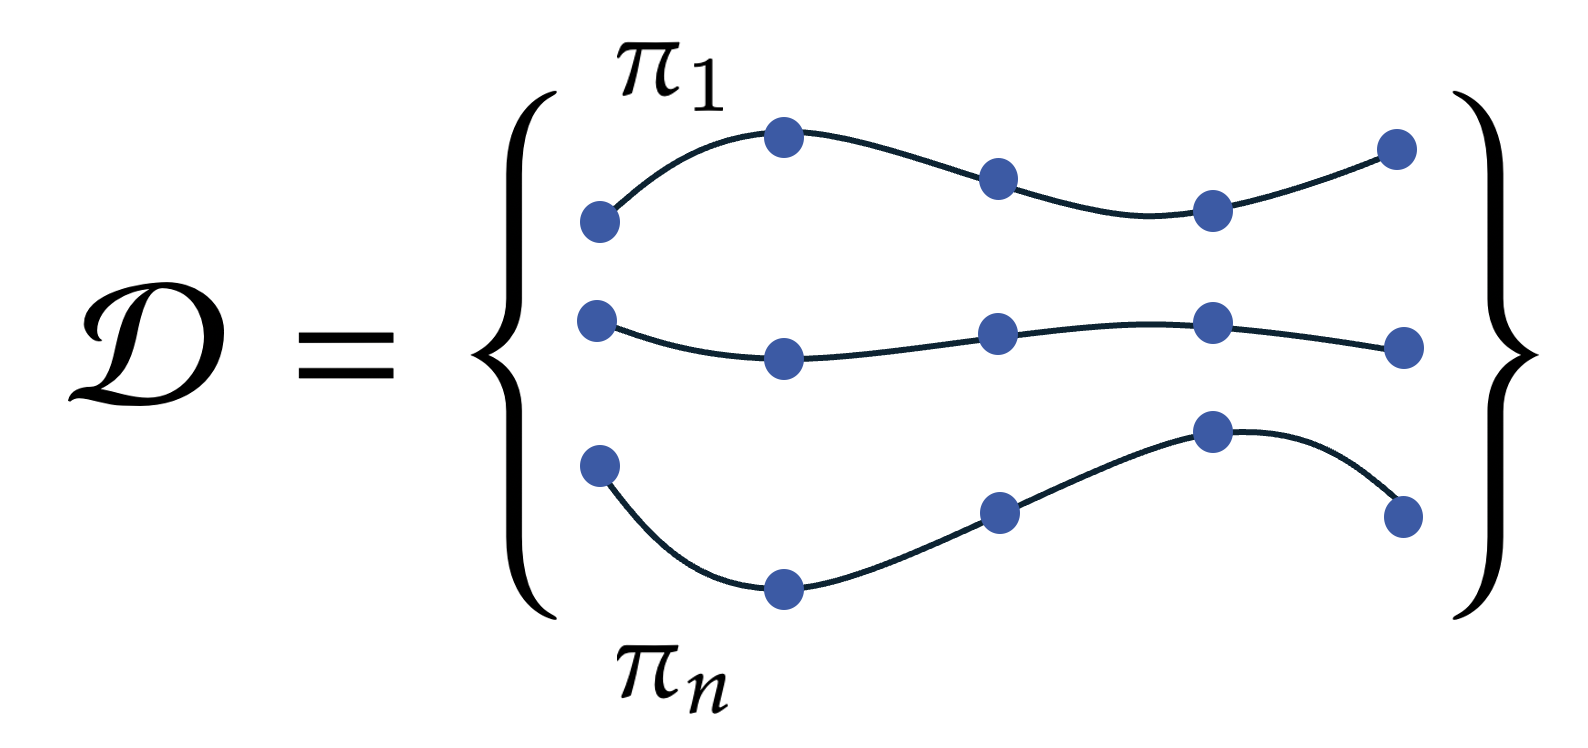
\includegraphics[scale=0.25]{figures/dataset.png}
\end{center}


% \begin{alertblock}{Goal}
%     Design a theoretically grounded algorithm for learning $\hat{f}\approx f^\star$ that is good for any reward functions.
% \end{alertblock}
\reffootnote{Introduction video by Bhavya Sukhija. NeurIPS 2023.}

\end{frame}


\begin{frame}{Problem Formulation (2/2)}


Our problem can be divided into two parts:
\begin{itemize}
    \item \textcolor{ETHRed}{Exploration (our focus!):} Collecting data by executing policies.
    \item Estimation: Building model from data.
\end{itemize}

\begin{block}{Well-Calibration Assumption}
    Given $n$ data, we can construct confidence intervals:
    \[
        \lvert f^\star_i(s,a) - {\color{ETHRed}\mu_{n,i}(s,a)} \rvert
            \leq {\color{ETHRed}\beta_n \sigma_{n,i}(s,a)} \quad \forall i\in[d],\ \text{w.h.p.},
    \]
    \begin{center}
    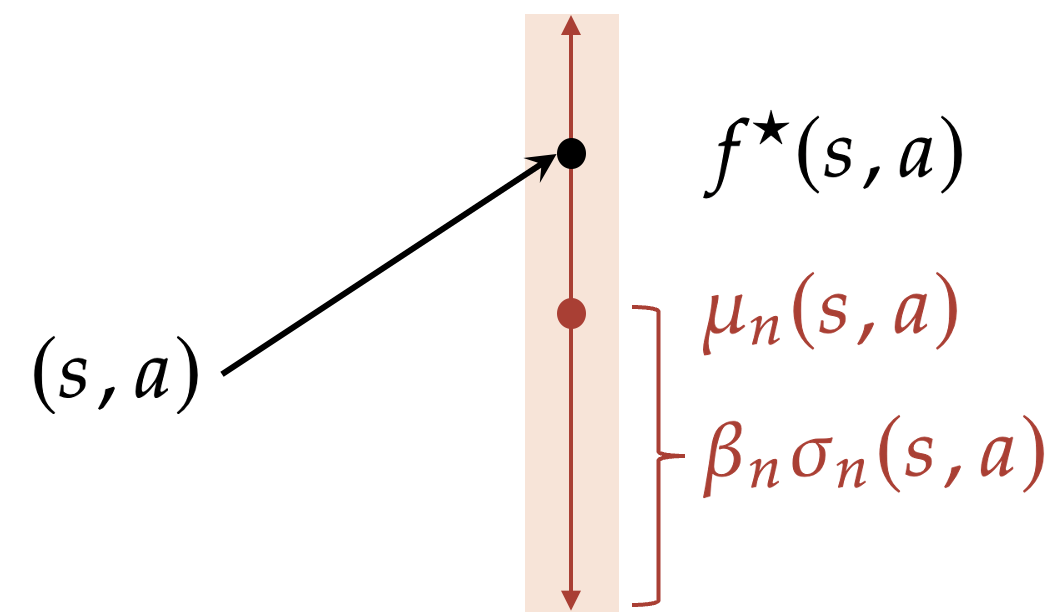
\includegraphics[scale=0.25]{figures/confidence_interval.png}
    \end{center}
\end{block}

\end{frame}


% \begin{frame}{Challenges}

% \end{frame}

% \begin{frame}{System Dynamics and Objective}
%     \begin{itemize}
%         \item Consider a discrete-time stochastic dynamical system:
%             \[ x_{k+1} = \mathalert{f^*(x_k, u_k)} + w_k \]
%             \begin{itemize}
%                 \item $x_k \in \mathcal{X}$: State
%                 \item $u_k \in \mathcal{U}$: Action
%                 \item $\mathalert{f^*}$: Unknown true dynamics function
%                 \item $w_k$: Noise (aleatoric uncertainty), e.g., $w_k \sim \mathcal{N}(0, \sigma^2 I)$
%             \end{itemize}
%         \pause
%         \item \textbf{Goal:} Learn a model $\hat{f}_N$ after $N$ episodes (each horizon $T$) that accurately approximates $f^*$ over the \textit{reachable state-action space} $\mathcal{R}$.
%             \[ \mathcal{R} = \{ (x, u) \mid \exists \pi, t<T \text{ s.t. } p(z_t = (x,u) \mid \pi, f^*) > 0 \} \]
%         \pause
%         \item \textbf{Measure of Success:} Reduction in \textit{epistemic uncertainty} (uncertainty about $f^*$) provided by a probabilistic model $(\mu_N, \sigma_N)$.
%         \item \textbf{Constraint:} Data is collected sequentially via trajectories $\tau_n = (x_0, u_0, x_1, ..., x_T)$, not arbitrary queries.
%     \end{itemize}
% \end{frame}

% \begin{frame}{Information-Theoretic Formulation}
%     \begin{itemize}
%         \item \textbf{Ideal Objective:} Maximize Mutual Information $I(f^*; \mathcal{D}_{1:N})$ between dynamics and collected data $\mathcal{D}_{1:N}$. Intractable.
%         \pause
%         \item \textbf{Greedy Episodic Approximation:} At each episode $n$, choose policy $\pi_n$ to maximize expected information gain from the *next* trajectory $\tau_n$:
%             \[ \max_{\pi \in \Pi} \mathbb{E}_{\tau^\pi} [ I(f^*_{\tau^\pi}; y_{\tau^\pi} | \mathcal{D}_{1:n-1}) ] \quad (*) \]
%             \begin{itemize}
%                 \item $f^*_{\tau^\pi}$: True dynamics values along trajectory $\tau^\pi$.
%                 \item $y_{\tau^\pi}$: Observed next states along $\tau^\pi$.
%                 \item $\mathcal{D}_{1:n-1}$: Data from previous episodes.
%                 \item Expectation is over noise $w_k$ and current uncertainty in $f^*$.
%             \end{itemize}
%         \pause
%         \item \textbf{Core Challenge of OPAX:} How to tractably approximate and optimize objective $(*)$ when $f^*$ is unknown?
%     \end{itemize}
% \end{frame}


\section{Related Work and Contributions}

\begin{frame}{Related Work: Active Learning}
    \renewcommand{\arraystretch}{1.25}
    \begin{table}[h]
        \centering
        \begin{tabular}{c|c|c}
        \toprule
          & Bandit Optimization & Our Problem \\
        \midrule
          Goal & $\displaystyle\max_{x} f^\star(x)$ & Find $\hat{f}\approx f^\star$ \\
          $f^\star$ & Objective & Dynamics \\
          State space & No & \color{ETHRed}{Continuous} \\
          % Action space & Continuous & Continuous \\
          Planning & No & \color{ETHRed}{Yes} \\
          Technique & \multicolumn{2}{c}{\color{ETHRed}{Optimism in the face of uncertainty}} \\
        \bottomrule
        \end{tabular}
        %\caption{Caption}
        %\label{tab:my_label}
    \end{table}

    \reffootnote{N.~Srinivas et al. ``Gaussian process optimization in the bandit setting: No regret and experimental design.'' ICML 2010. (The 1st presentation today!)}
\end{frame}


\begin{frame}{Related Work: Maximum Entropy RL}

    What about collecting data by maximum entropy or entropy-regularized RL?
    
    $$
    \max_{\pi} H\left(d^{\pi}_\mu\right), \quad
        \max_{\pi} \mathbb{E}\left[ \sum_{t=0}^\infty \gamma^t (r(s_t, a_t) - \beta\log\pi(a_t|s_t)) \,\middle|\, s_0\sim \mu , \pi \right].
    $$
    
    \begin{itemize}
        \item \textcolor{ETHRed}{No guarantee} for arbitrary reward functions in downstream tasks.
    \end{itemize}

    \reffootnote{E.~Hazan et al. ``Provably efficient maximum entropy exploration.'' ICML 2019. (The 3rd presentation today!)\\
    B.~Eysenbach and S.~Levine. ``Maximum entropy RL (provably) solves some robust RL problems.'' ICLR 2022.}
\end{frame}


\begin{frame}{Related Work: Reward-Free RL}

    \begin{itemize}
        % \item For every ``non-negligible'' state-action pair, collect data by optimism in the face of uncertainty.
        %\item Sample complexity is $\text{poly}(\lvert\mathcal{S}\rvert, \lvert\mathcal{A}\rvert, T)$ in the tabular setting.
        \item Study this problem in tabular settings or impose \textcolor{ETHRed}{structural assumptions on values function and transitions}.
        % \item In the continuous setting, existing functional approximation results
        % \begin{itemize}
        %     \item \normalsize require \textcolor{ETHRed}{structural assumptions on values function and transitions}, and
        %     \item \normalsize may suffer from \textcolor{ETHRed}{exponential} sample complexity lower bound.
        % \end{itemize}
        \item No practical algorithms.
    \end{itemize}

    \reffootnote{C.~Jin et al. ``Reward-free exploration for reinforcement learning.'' ICML 2020.\\
    R.~Wang et al. ``On reward-free reinforcement learning with linear function approximation.'' NeurIPS 2020.\\
    J.~Chen et al. ``On the statistical efficiency of reward-free exploration in non-linear RL.'' NeurIPS 2022.}
\end{frame}


\begin{frame}{Contributions}

    \begin{itemize}
        \item Propose OpAX, a practical algorithm for learning non-linear dynamics with \textcolor{ETHRed}{continuous} state-action spaces and \textcolor{ETHRed}{without} structural assumptions.
        \item In this setting, OpAX is the \textcolor{ETHRed}{first} algorithm to have a theoretical guarantee for a rich family of nonlinear dynamics. 
    \end{itemize}
\end{frame}


% --- Section 3: Methodology ---
\section{Methodology: Optimism in Information Space}

\begin{frame}{How OPAX Works: Information as Reward \hl{ben}}
    \textbf{Key Idea:} Transform exploration into a sequential decision problem with intrinsic rewards
    
    \vspace{0.5em}
    \begin{columns}[T]
        \begin{column}{0.5\textwidth}
            \textbf{1. Model Uncertainty}
            \begin{itemize}
                \item Learn dynamics with uncertainty: $(\mu_n, \sigma_n)$
                \item GP or Neural Network Ensemble
            \end{itemize}
            
            \vspace{0.5em}
            \textbf{2. Information Reward}
            \[ r_{\text{info}}(s,a) = \sum_{j} \log\left(1 + \frac{\sigma_{n,j}^2(s,a)}{\sigma_w^2}\right) \]
            \centering
            \small High reward = high uncertainty
        \end{column}
        \begin{column}{0.25\textwidth}
            \textbf{3. Exploration Strategy}
            \begin{block}{Traditional RL}
                \centering
                Maximize task reward \\
                $\Downarrow$ \\
                Biased exploration \\
            \end{block}
        \end{column}
        \begin{column}{0.25\textwidth}
            \begin{block}{OPAX}
                \centering
                Maximize \alert{information gain} \\
                $\Downarrow$ \\
                Comprehensive exploration
            \end{block}
        \end{column}
    \end{columns}
    
    \vspace{0.5em}
    \begin{block}{Why Information Gain?}
        \begin{itemize}
            \item Principled: Rooted in Bayesian experimental design
            \item Task-agnostic: No bias towards specific rewards
            \item Diminishing returns: Log ensures convergence
        \end{itemize}
    \end{block}
\end{frame}

\begin{frame}{Step 1: Information-Theoretic Objective \hl{ben}}
    \textbf{Ideal Goal:} Maximize mutual information between dynamics $f^*$ and collected data
    
    \vspace{0.5em}
    \textbf{Greedy Episodic Approximation:} At episode $n$, choose policy to maximize expected information gain:
    \begin{align}
        \pi_n^* = \argmax_{\pi \in \Pi} \mathbb{E}_{\tau^\pi}\left[I\left(f^*_{\tau^\pi}; y_{\tau^\pi} \mid \mathcal{D}_{1:n-1}\right)\right]
    \end{align}
    
    where:
    \begin{itemize}
        \item $f^*_{\tau^\pi} = (f^*(z_{0}), \ldots, f^*(z_{T-1}))$ - true dynamics along trajectory
        \item $y_{\tau^\pi} = (y_{0},\ldots, y_{T-1})$ - observed next states  
        \item $\mathcal{D}_{1:n-1}$ - data from previous episodes
    \end{itemize}
    
    \vspace{0.5em}
    \begin{alertblock}{Challenge}
        This objective is \textcolor{red}{intractable} in general. Need tractable approximation.
    \end{alertblock}
\end{frame}

\begin{frame}{Step 2: Tractable Upper Bound \hl{ben}}
    \begin{lemma}[Information gain upper bound]
        For Gaussian noise $w \sim \mathcal{N}(0, \sigma^2 I)$ and epistemic uncertainty $\sigma_{n-1}$:
        \begin{align}
            I\left(f^*_{\tau^\pi}; y_{\tau^\pi} \mid \mathcal{D}_{1:n-1}\right) &\leq \frac{1}{2} \sum_{t=0}^{T-1} \sum_{j=1}^{d_x} \log \left(1 + \frac{\sigma_{n-1, j}^2(z_t)}{\sigma^2}\right)
        \end{align}
    \end{lemma}
    
    \vspace{0.5em}
    \textbf{Tractable Exploration Objective:} Maximize the upper bound
    \begin{align}
        \pi_n^* = \argmax_{\pi \in \Pi} \mathbb{E}_{\tau^\pi}\left[\sum_{t=0}^{T-1} \sum_{j=1}^{d_x} \underbrace{\frac{1}{2}\log \left(1 + \frac{\sigma_{n-1, j}^2(x_t, \pi(x_t))}{\sigma^2}\right)}_{r_{\text{info}}(x_t, \pi(x_t))}\right]
    \end{align}
    
    subject to: $x_{t+1} = f^*(x_t, \pi(x_t)) + w_t$
    
    \begin{block}{Interpretation}
        Collect data where model is most uncertain $\Rightarrow$ maximal information gain
    \end{block}
\end{frame}

\begin{frame}{Step 3: The Optimism Challenge \hl{ben}}
    \textbf{Problem:} The planning objective requires knowing $f^*$, but $f^*$ is unknown!
    
    \vspace{0.5em}
    \textbf{Naive Solution:} Use mean estimate $\mu_{n-1}$ instead of $f^*$
    \begin{align}
        x_{t+1} = \mu_{n-1}(x_t, \pi(x_t)) + w_t
    \end{align}
    
    \textcolor{red}{\textbf{Issue:}} Mean planner may believe uncertain regions are unreachable
    
    \vspace{0.5em}
    \textbf{OPAX Solution:} \alert{Optimism in the face of uncertainty}
    
    Define confidence set of plausible dynamics:
    \begin{align}
        \mathcal{F}_{n-1} = \left\{ \tilde{f} \mid \|\tilde{f}(z) - \mu_{n-1}(z)\| \leq \beta_{n-1} \sigma_{n-1}(z) \,\forall z \right\}
    \end{align}
    
    \textbf{Key Insight:} Plan assuming the \alert{most optimistic} dynamics for reaching uncertain states
\end{frame}

\begin{frame}{Step 4: Optimistic Planning Formulation \hl{ben}}
    \textbf{OPAX Optimistic Objective:}
    \begin{align}
        \pi_n, \eta_n = \argmax_{\pi \in \Pi, \eta \in \Xi} \mathbb{E}_{\tau^{\pi,\eta}}\left[\sum_{t=0}^{T-1} \sum_{j=1}^{d_x} \log \left(1 + \frac{\sigma_{n-1, j}^2(\tilde{x}_t, \pi(\tilde{x}_t))}{\sigma^2}\right)\right]
    \end{align}
    
    subject to: 
    \begin{align}
        \tilde{x}_{t+1} = \mu_{n-1}(\tilde{x}_t, \pi(\tilde{x}_t)) + \beta_{n-1} \sigma_{n-1}(\tilde{x}_t, \pi(\tilde{x}_t)) \eta(\tilde{x}_t) + w_t
    \end{align}
    
    where $\Xi = \{\eta: \mathcal{X} \to [-1, 1]^{d_x}\}$ is the space of \alert{hallucination policies}
    
    \vspace{0.5em}
    \begin{itemize}
        \item $\eta(\tilde{x}_t)$ picks the most optimistic transition within confidence bounds
        \item Equivalent to $\max_{\tilde{f} \in \mathcal{F}_{n-1}} \mathbb{E}_{\tau^\pi | \tilde{f}}[\text{info reward}]$
        \item Guarantees $J_n(\pi^*) \leq J_n(\pi_n, \eta_n)$ w.h.p. (optimistic estimate)
    \end{itemize}
    
    \begin{alertblock}{Implementation}
        Solve as optimal control with extended action space $(\pi, \eta)$ using MPC or SAC
    \end{alertblock}
\end{frame}

% --- Section 4: Theoretical Contributions ---
\section{Theoretical Guarantees}


% \begin{frame}{Benefit of Optimism}

% Recall
% \begin{align*}
%     \pi^\star &\in \argmax_{\pi} J_n(\pi),
%     &&s_{t+1} = f^\star(s_t, a_t) + w_t \\
%     (\pi_{n}, \eta_{n}) &\in \argmax_{\substack{\pi\\ {\color{ETHRed}\eta:\mathcal{S}\to[-1,1]^d}}} J_n(\pi,\eta),
%     &&s_{t+1} = \mu_{n-1}(s_t,a_t) + {\color{ETHRed}\eta(s_t)}\beta_{n-1}\sigma_{n-1}(s_t,a_t) +w_t.
% \end{align*}

% \begin{lemma}[Optimistic Estimate]
% $J_n(\pi^\star) \leq J_n(\pi_n, \eta_n)$ w.h.p. 
% \end{lemma}

% % Follows from well-calibration assumption
% % \[
% %     \lvert f^\star_i(s,a) - \mu_{n,i}(s,a) \rvert
% %     \leq \beta_n \sigma_{n,i}(s,a) \quad \forall i\in[d],\ \text{w.h.p.}
% % \]
% \end{frame}

\begin{frame}{Assumptions}

    % \begin{block}{Well Calibration}
    %     Given $n$ data-points, we can construct a confidence interval:
    %     \[
            
    %     \]
    % \end{block}

    \begin{block}{Regularity of the Dynamics}
        $f^\star$ lies in a RKHS with kernel $k$ and $\lVert f^\star \rVert \leq 1$.
    \end{block}

    Recall
    \[
        \gamma_n(k) = \max_{\mathcal{D}_1,\ldots,\mathcal{D}_n} \log\det(I + K_n)
    \]
    and
    \[
        \gamma_n(\text{linear}), \gamma_n(\text{RBF}) \asymp \text{polylog}(nT).
    \]

    % $\mathcal{GP}(0,k)$ is well calibrated:
    %     \[
    %         \lvert f^\star_i(s,a) - \mu_{n,i}(s,a) \rvert
    %         \leq \beta_n\sigma_{n,i}(s,a) \quad \forall i\in[d],\ \text{w.h.p.},
    %     \]
    %     with
    %     \[
    %         \beta_n = \text{poly}(B,\sigma,\gamma_n(k)),
    %         \quad
    %         \gamma_n(k) = \max_{\mathcal{D}_1,\ldots,\mathcal{D}_n} \log\det(I + \sigma^{-2}K_n).
    %     \]
    
    \reffootnote{N.~Srinivas et al. ``Gaussian process optimization in the bandit setting: No regret and experimental design.'' ICML 2010. (The 1st presentation today!)}
    % \reffootnote{Rothfuss et al. ``Hallucinated adversarial control for conservative offline policy evaluation.'' UAI 2023.}
\end{frame}


\begin{frame}{Main Guarantee}
    \begin{theorem}[Informal]
        If we use $\mathcal{GP}(0,k)$ to build well-calibrated confidence intervals, then w.h.p.
        \[
            \E_{\pi} \bigg[ \underbrace{
            \max_{t} \lVert \sigma_n(s_t,a_t)\rVert^2_2
            }_{
            \substack{\color{ETHRed}\text{maximum uncertainty}\\\color{ETHRed}\text{along the trajectory}}
            } \bigg]
            \leq
            \text{poly}(T)
            \cdot \frac{\gamma_n(k)}{\sqrt{n}},
            \quad\forall\pi,\ \forall n\in\mathbb{N}.
        \]
    \end{theorem}
    % \begin{itemize}
    %     \item $\gamma_n(\text{linear})\asymp d\log (nT)$.
    %     \item $\asymp \log^{d+1}(nT)$.
    % \end{itemize}
    
    For linear and RBF kernels,
    \[
        \lim_{n\to\infty}\sigma_n(s, a)\to 0.
    \]
    
\end{frame}


\begin{frame}{Zero-Shot Performance}

\begin{corollary}[Informal]
    Consider an RL problem with a known bounded reward:
    \[
        \argmax_{\pi} R(\pi), \quad
        s_{t+1} = f^\star(s_t,a_t) + w_t.
    \]
    If
    $n \gtrsim \mathrm{poly}(d,T,\varepsilon^{-1},\gamma_n(k))$,
    then
    \[
        \max_{\pi} R(\pi) - R(\hat{\pi}) \leq \varepsilon,
    \]
    where
    \[
    \hat{\pi} \in \argmax_{\pi} {\color{ETHRed}\min_{\eta}{}} R(\pi,\eta),\quad
        s_{t+1} = \mu_n(s_t,a_t) + \eta(s_n)\beta_n\sigma_n(s_t,a_t) +w_t.
    \]
\end{corollary}
% NB: Can we find/approximate $\hat{\pi}$ efficiently?
\end{frame}



% \begin{frame}{Convergence and Regret Guarantees}
%     \begin{itemize}
%         \item OPAX provides theoretical guarantees for active learning of dynamics.
%         \pause
%         \item \textbf{General Models (Theorem 1):}
%         \begin{itemize}
%             \item Under valid confidence bounds (Assumption 1), relates total information gain achieved by OPAX to the sum of uncertainties encountered.
%             \item Justifies optimism: Optimistic planner achieves $\geq$ info gain than mean planner (Corollary 1).
%         \end{itemize}
%         \pause
%         \item \textbf{Gaussian Process Dynamics (Theorem 2):}
%         \begin{itemize}
%             \item Assume $f^*$ in RKHS $\mathcal{H}_k$, model with GP, noise assumptions.
%             \item Bounds sum of squared epistemic uncertainties over $N$ episodes ($NT$ steps):
%                 \[ \sum_{n=1}^N \mathbb{E} \left[ \sum_{t=0}^{T-1} \sigma_{n-1}^2(x_{n,t}, u_{n,t}) \right] \leq \mathcal{O}(\beta_N \mathalert{\gamma_{NT}(k)}) \]
%                 ($\gamma_{NT}(k)$ = max information gain for kernel $k$ with $NT$ samples).
%             \item For common kernels (RBF, Linear), $\gamma_{NT}(k) = \mathcal{O}(\text{polylog}(NT))$.
%             \item Implies average uncertainty $\frac{1}{NT}\sum \mathbb{E}[\sigma^2]$ decays.
%             \item Proves \textit{almost sure convergence}: $\mathalert{\sigma_n(z) \xrightarrow{a.s.} 0}$ as $n \to \infty$ for all reachable $z \in \mathcal{R}$.
%         \end{itemize}
%         \pause
%         \item \textbf{Significance:} First sample complexity bounds and convergence guarantees for active GP dynamics learning in this setting.
%     \end{itemize}
% \end{frame}

% \begin{frame}{Link to Zero-Shot Performance}
%     \begin{itemize}
%         \item \textbf{Goal:} Show that reducing epistemic uncertainty $\sigma_N$ leads to good performance on downstream tasks.
%         \pause
%         \item \textbf{Result (Corollary 7):}
%         \begin{itemize}
%             \item Consider a downstream task with bounded cost function $c(x,u)$.
%             \item Let $J^*(\pi)$ be the cost using true dynamics $f^*$.
%             \item Let $\hat{J}_N(\pi)$ be the cost using the learned mean model $\mu_N$.
%             \item The difference in performance (suboptimality due to model error) is bounded:
%                 \[ | J^*(\pi) - \hat{J}_N(\pi) | \leq \mathcal{O}\left( \mathbb{E}_{\tau^\pi | f^*} \left[ \sum_{t=0}^{T-1} \beta \sigma_N(x_t, u_t) \right] \right) \]
%                 (Simplified expression)
%         \end{itemize}
%         \pause
%         \item \textbf{Implication:} If OPAX drives uncertainty $\sigma_N$ low across the reachable space $\mathcal{R}$, policies planned with the learned model $\mu_N$ will perform well (close to optimal) on new tasks within $\mathcal{R}$ \textit{without} further learning (zero-shot).
%     \end{itemize}
% \end{frame}

% --- Section 5: Empirical Evaluation ---
\section{Empirical Evaluation}

\begin{frame}{Experiments: Reduction in Epistemic Uncertainty (ok) \hl{ben}}
    \centering
    \textbf{Does OPAX achieve its goal of reducing uncertainty everywhere?}
    
    \vspace{0.1em}
    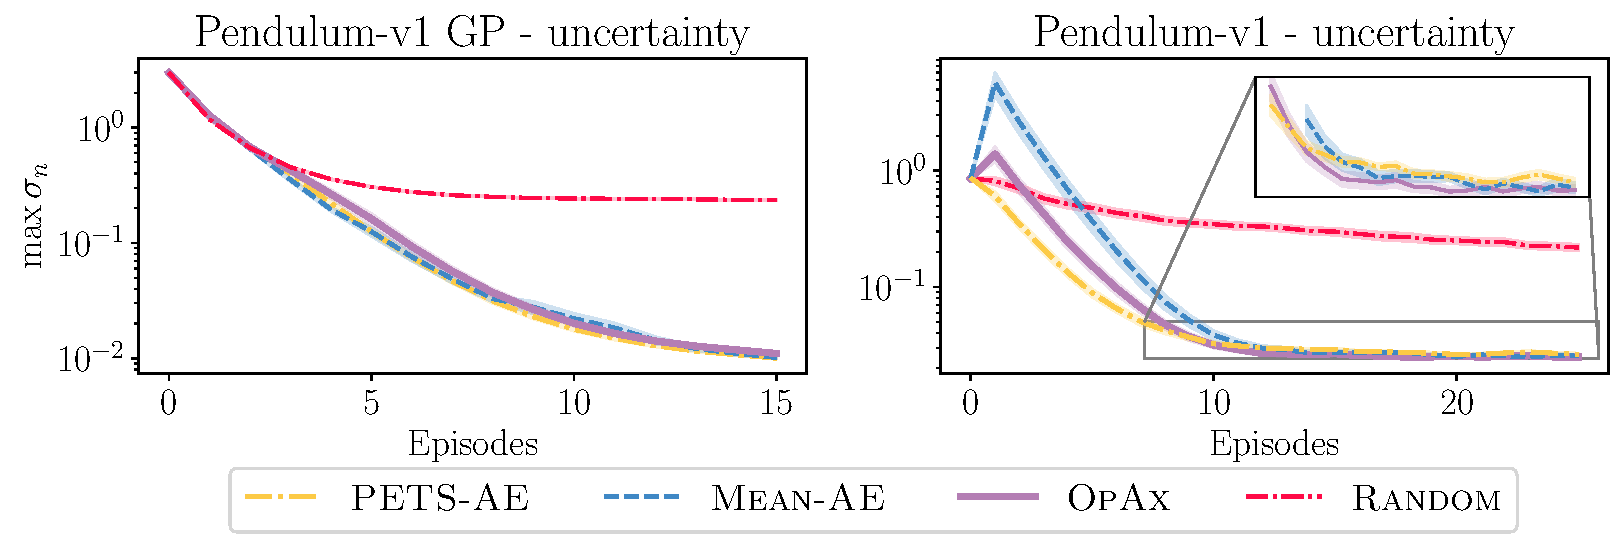
\includegraphics[width=0.75\linewidth]{figures/uncertainty_plotvalidation_eps_std_max.pdf}
    
    \vspace{0.1em}
    \begin{columns}[T]
        \begin{column}{0.48\textwidth}
            \textbf{Key Findings:}
            \begin{itemize}
                \item OPAX reduces uncertainty much than random
                \item All active methods outperform random baseline
                \item Validates theoretical convergence guarantees
            \end{itemize}
        \end{column}
        \begin{column}{0.48\textwidth}
            \textbf{Implications:}
            \begin{itemize}
                \item Information-driven exploration works in practice
                \item Both GP and PE models benefit from active exploration
                \item Optimism provides slight edge over mean planning
            \end{itemize}
        \end{column}
    \end{columns}
\end{frame}

\begin{frame}{Experimental Setup and Baselines \hl{ben}}
    \begin{columns}[T]
        \begin{column}{0.5\textwidth}
            \textbf{Test Environments:}
            \begin{itemize}
                \item Pendulum, MountainCar
                \item Reacher, Swimmer, Cheetah  
                \item Fetch Manipulation (58D)
            \end{itemize}
            
            \vspace{0.5em}
            \textbf{Key Comparisons:}
            \begin{itemize}
                \item \textbf{OPAX} vs \textbf{H-UCRL} (task-specific SOTA)
                \item \textbf{OPAX} vs other active exploration methods
            \end{itemize}
        \end{column}
        \begin{column}{0.5\textwidth}
            \textbf{Evaluation Protocol:}
            \begin{enumerate}
                \item Train models with different exploration strategies
                \item Test on both \alert{seen} and \alert{unseen} tasks
                \item Measure zero-shot performance
            \end{enumerate}
            
            \vspace{0.5em}
            \textbf{Models:} GP (theory) \& PE (scale)\\
            \textbf{Planning:} MPC or SAC
        \end{column}
    \end{columns}
\end{frame}

\begin{frame}{Experiments: Learning and Zero-Shot Generalization \hl{ben}}

    \begin{itemize}
         \item \texttt{OpAx} performs \alert{on par} with \texttt{H-UCRL} on trained tasks
         \item \texttt{OpAx} \alert{outperforms} \texttt{H-UCRL} on some unseen tasks
     \end{itemize}

\end{frame}

\begin{frame}{Experiments: Learning and Zero-Shot Generalization \hl{ben}}
    \vspace{-0.2in}
    \begin{itemize}
         \item \texttt{OpAx} performs \alert{on par} with \texttt{H-UCRL} on trained tasks
         \item \texttt{OpAx} \alert{outperforms} \texttt{H-UCRL} on some unseen tasks
     \end{itemize}
    \begin{columns}[T] % Align tops
         \begin{column}{0.6\textwidth}
            Evaluation (\fcolorbox{black}{black}{\rule{0pt}{1pt}\rule{1pt}{0pt}}\:: \texttt{H-UCRL}, \fcolorbox{black}{Fuchsia}{\rule{0pt}{1pt}\rule{1pt}{0pt}}\:: \texttt{OpAx}, \fcolorbox{black}{red}{\rule{0pt}{1pt}\rule{1pt}{0pt}}\:: Random):\vspace{-0.2in}
            \begin{figure}
              \centering
              \subfloat[Trained task\label{fig:a}]{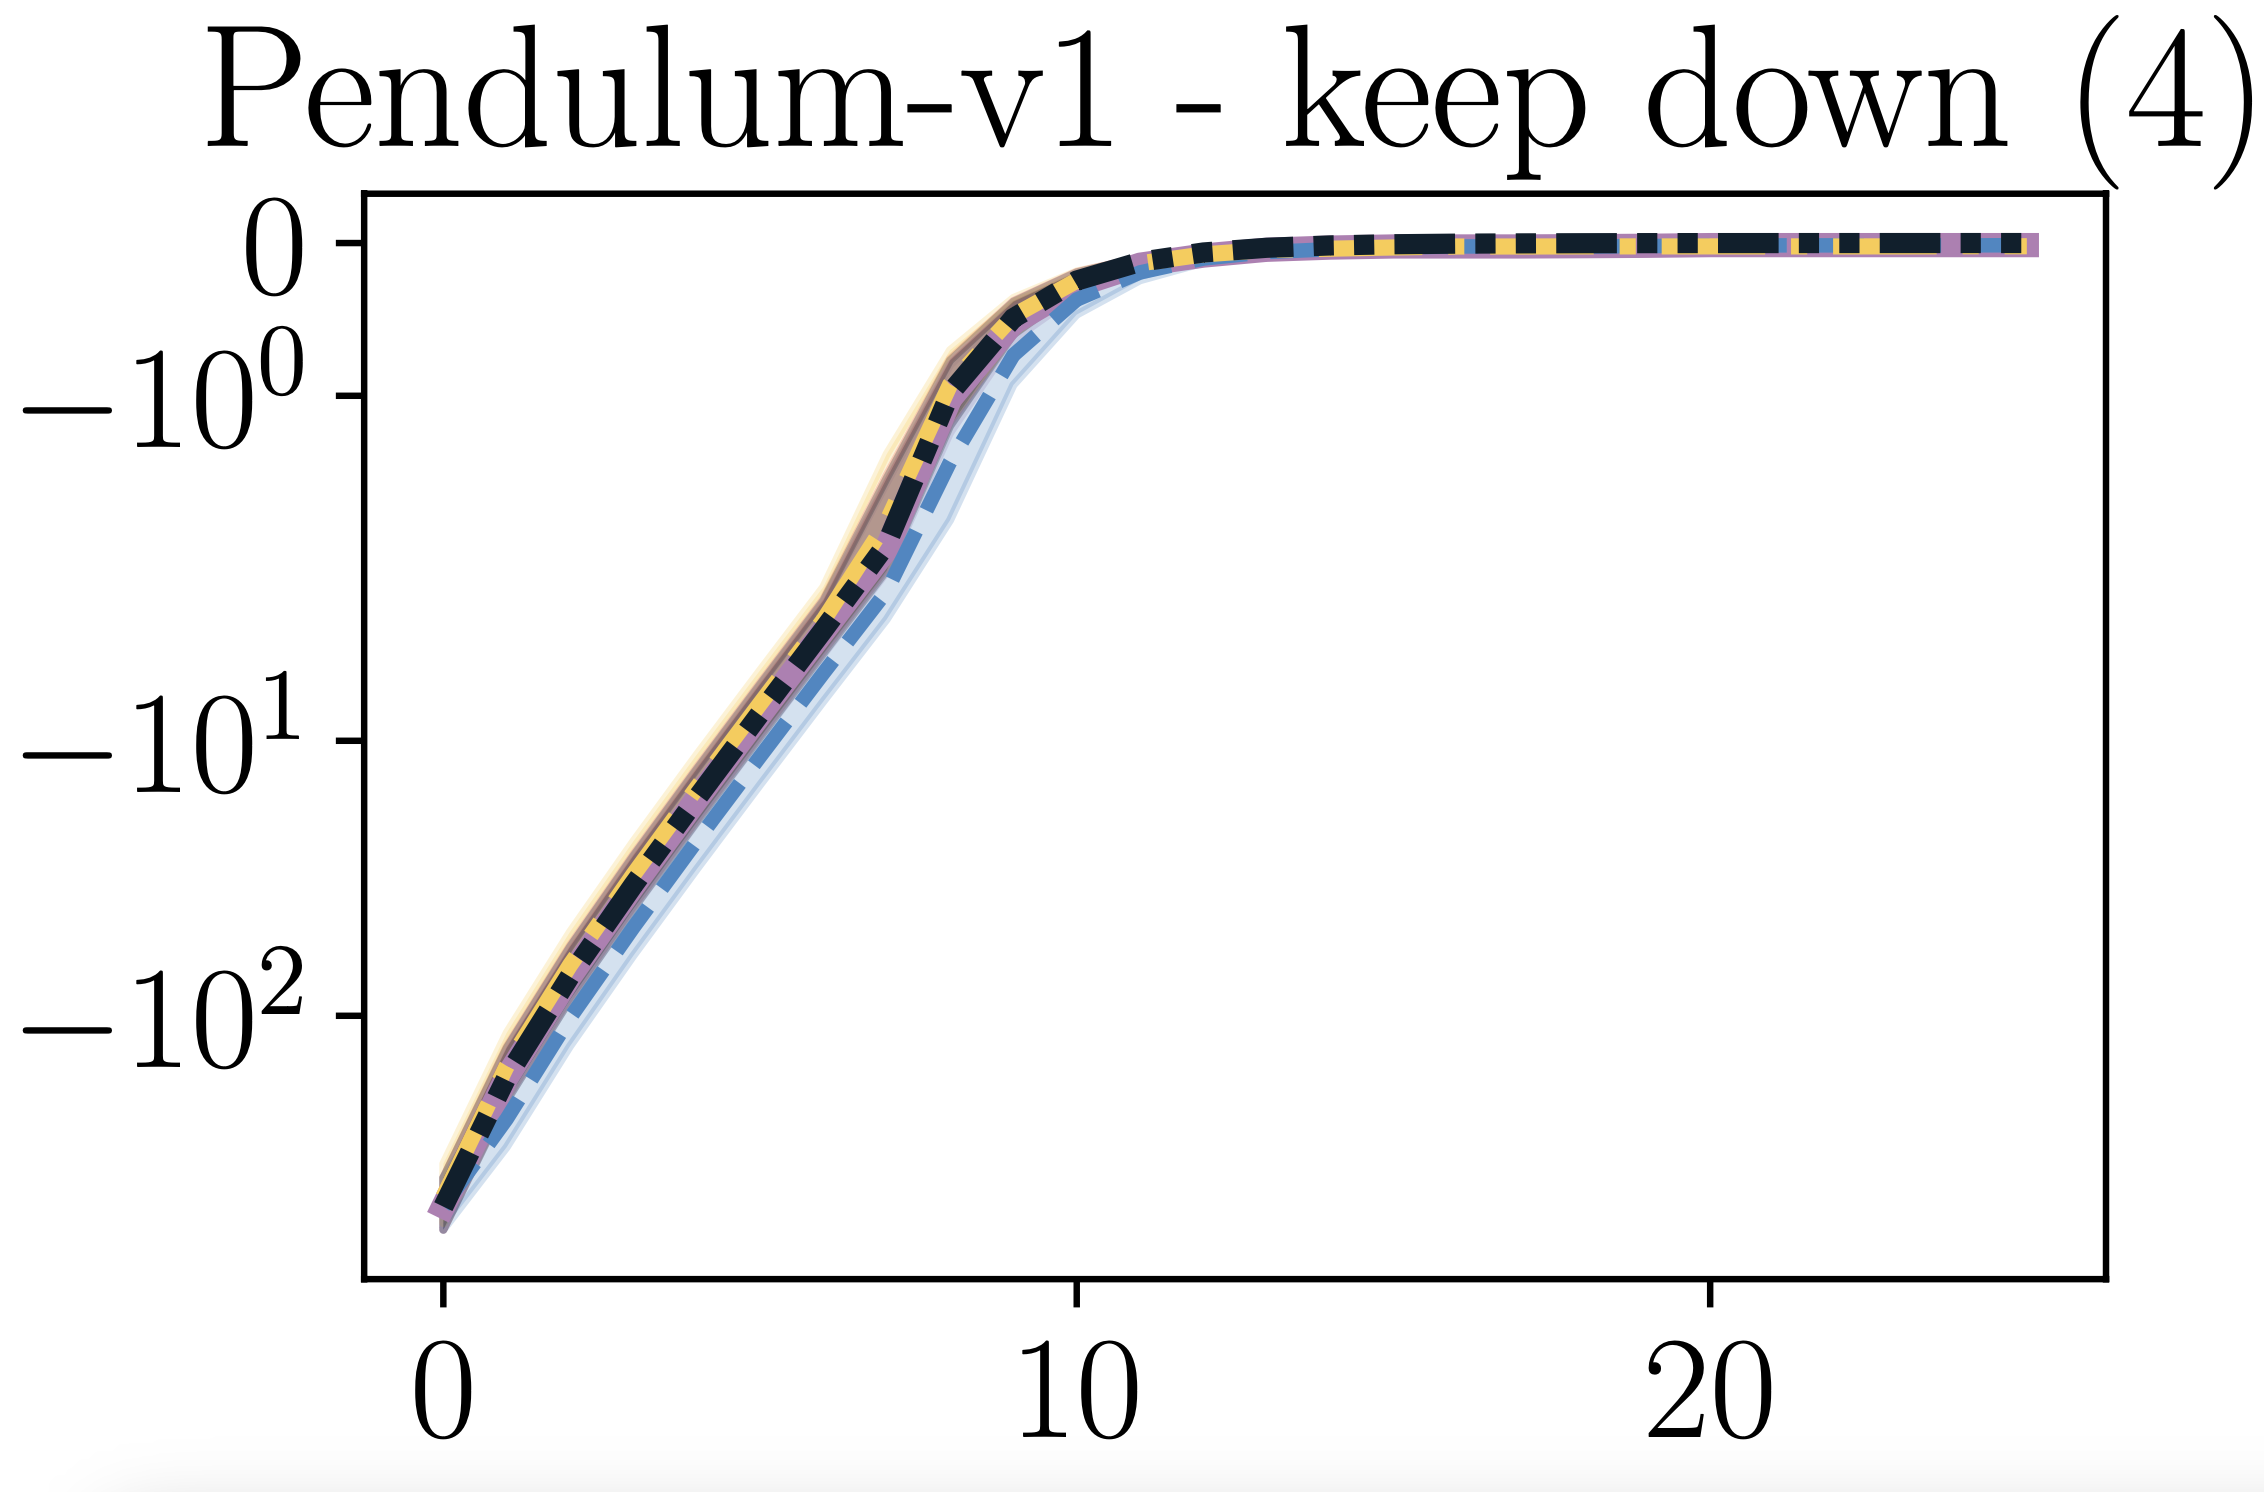
\includegraphics[width=0.37\linewidth]{figures/pendulum-keep-down.png}}
        
              \subfloat[Zero-shot task\label{fig:b}]{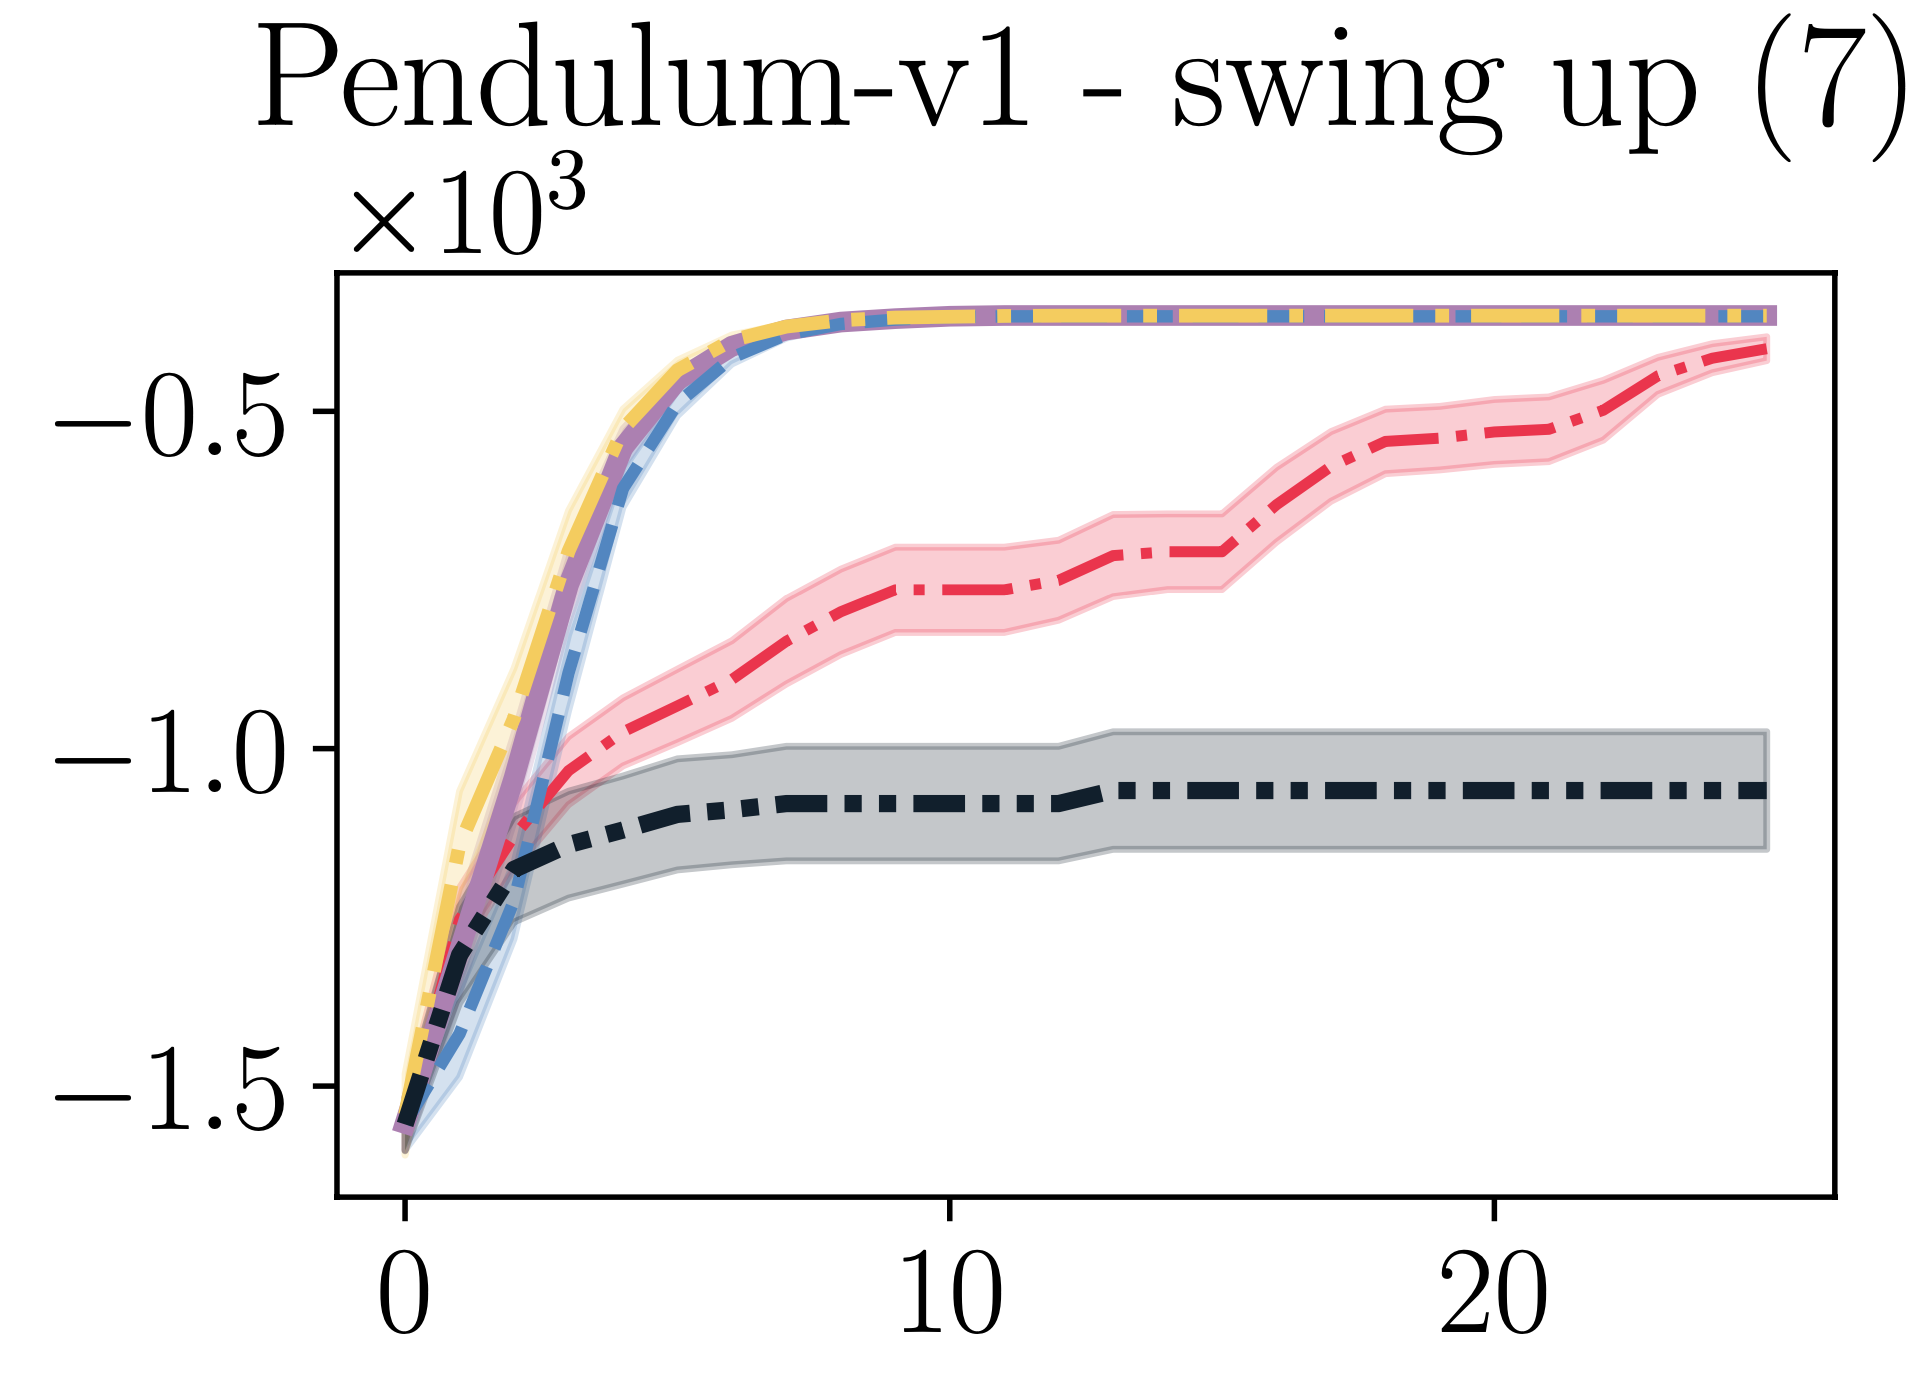
\includegraphics[width=0.37\linewidth]{figures/zero-shot-pendulum-swing-up.png}}
            %\caption{Evaluation}
            \label{fig:1}
            \end{figure}
         \end{column}
         \begin{column}{0.4\textwidth}
            Zero-shot swing up task:\vspace{-0.2in}
            \begin{figure}
              \centering
              \subfloat[\texttt{H-UCRL}\label{fig:a}]{\movie[label=false,height=0.37\linewidth,width=0.37\linewidth]{(play)}{videos/hucrl-zero-shot-swingup-4.mov}}
        
              \subfloat[\texttt{OpAx}\label{fig:b}]{\movie[label=false,height=0.37\linewidth,width=0.37\linewidth]
                {(play)}{videos/opax-zero-shot-swingup-4.mov}}
            %\caption{Evaluation}
            \label{fig:1}
            \end{figure}
         \end{column}
     \end{columns}

\end{frame}

\begin{frame}{Experiments: Comprehensive Downstream Task Performance \hl{ben}}
    \centering
    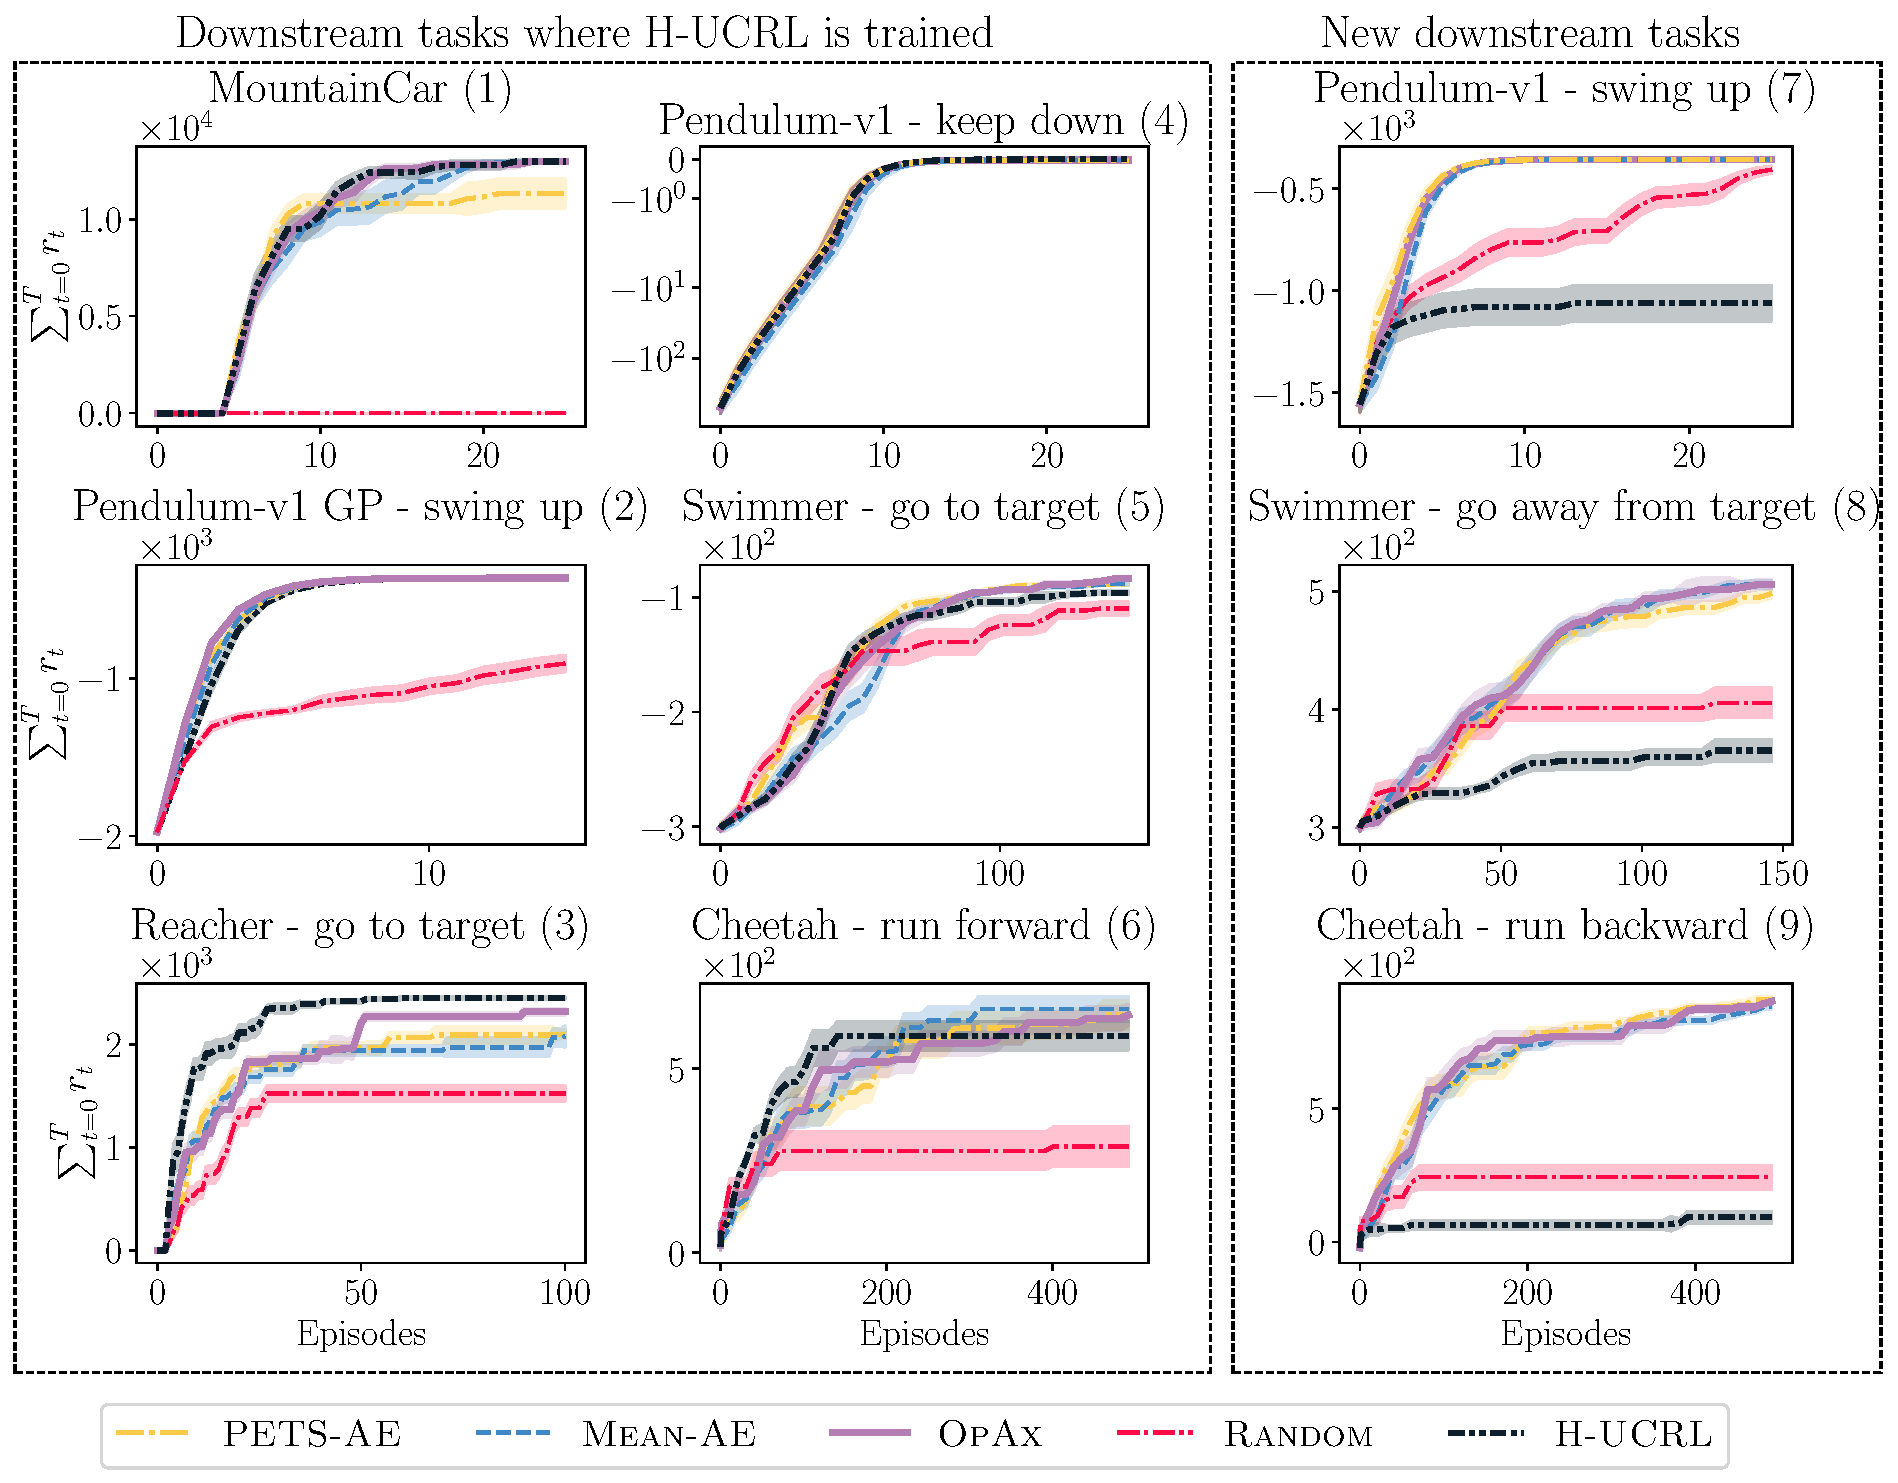
\includegraphics[width=0.5\linewidth]{figures/results_plot_with_hucrlreward_task_1.pdf}
    
    \begin{itemize}
        \item \textbf{OPAX} consistently performs well across all environments
        \item On par with \textbf{H-UCRL} on trained tasks (1-6)
        \item \textbf{Outperforms H-UCRL} on unseen/new tasks (7-9) by a large margin
        \item \textbf{Random} baseline struggles, especially on MountainCar
    \end{itemize}
\end{frame}

\begin{frame}{Experiments: High-Dimensional Object Manipulation \hl{ben}}
    \begin{columns}[T]
        \begin{column}{0.3\textwidth}
            \textbf{Fetch Pick \& Place Construction}
            \begin{itemize}
                \item 7-DoF robot arm
                \item Four 6-DoF blocks
                \item 58-dim state space
                \item 4-dim actions
            \end{itemize}
            \vspace{0.5em}
            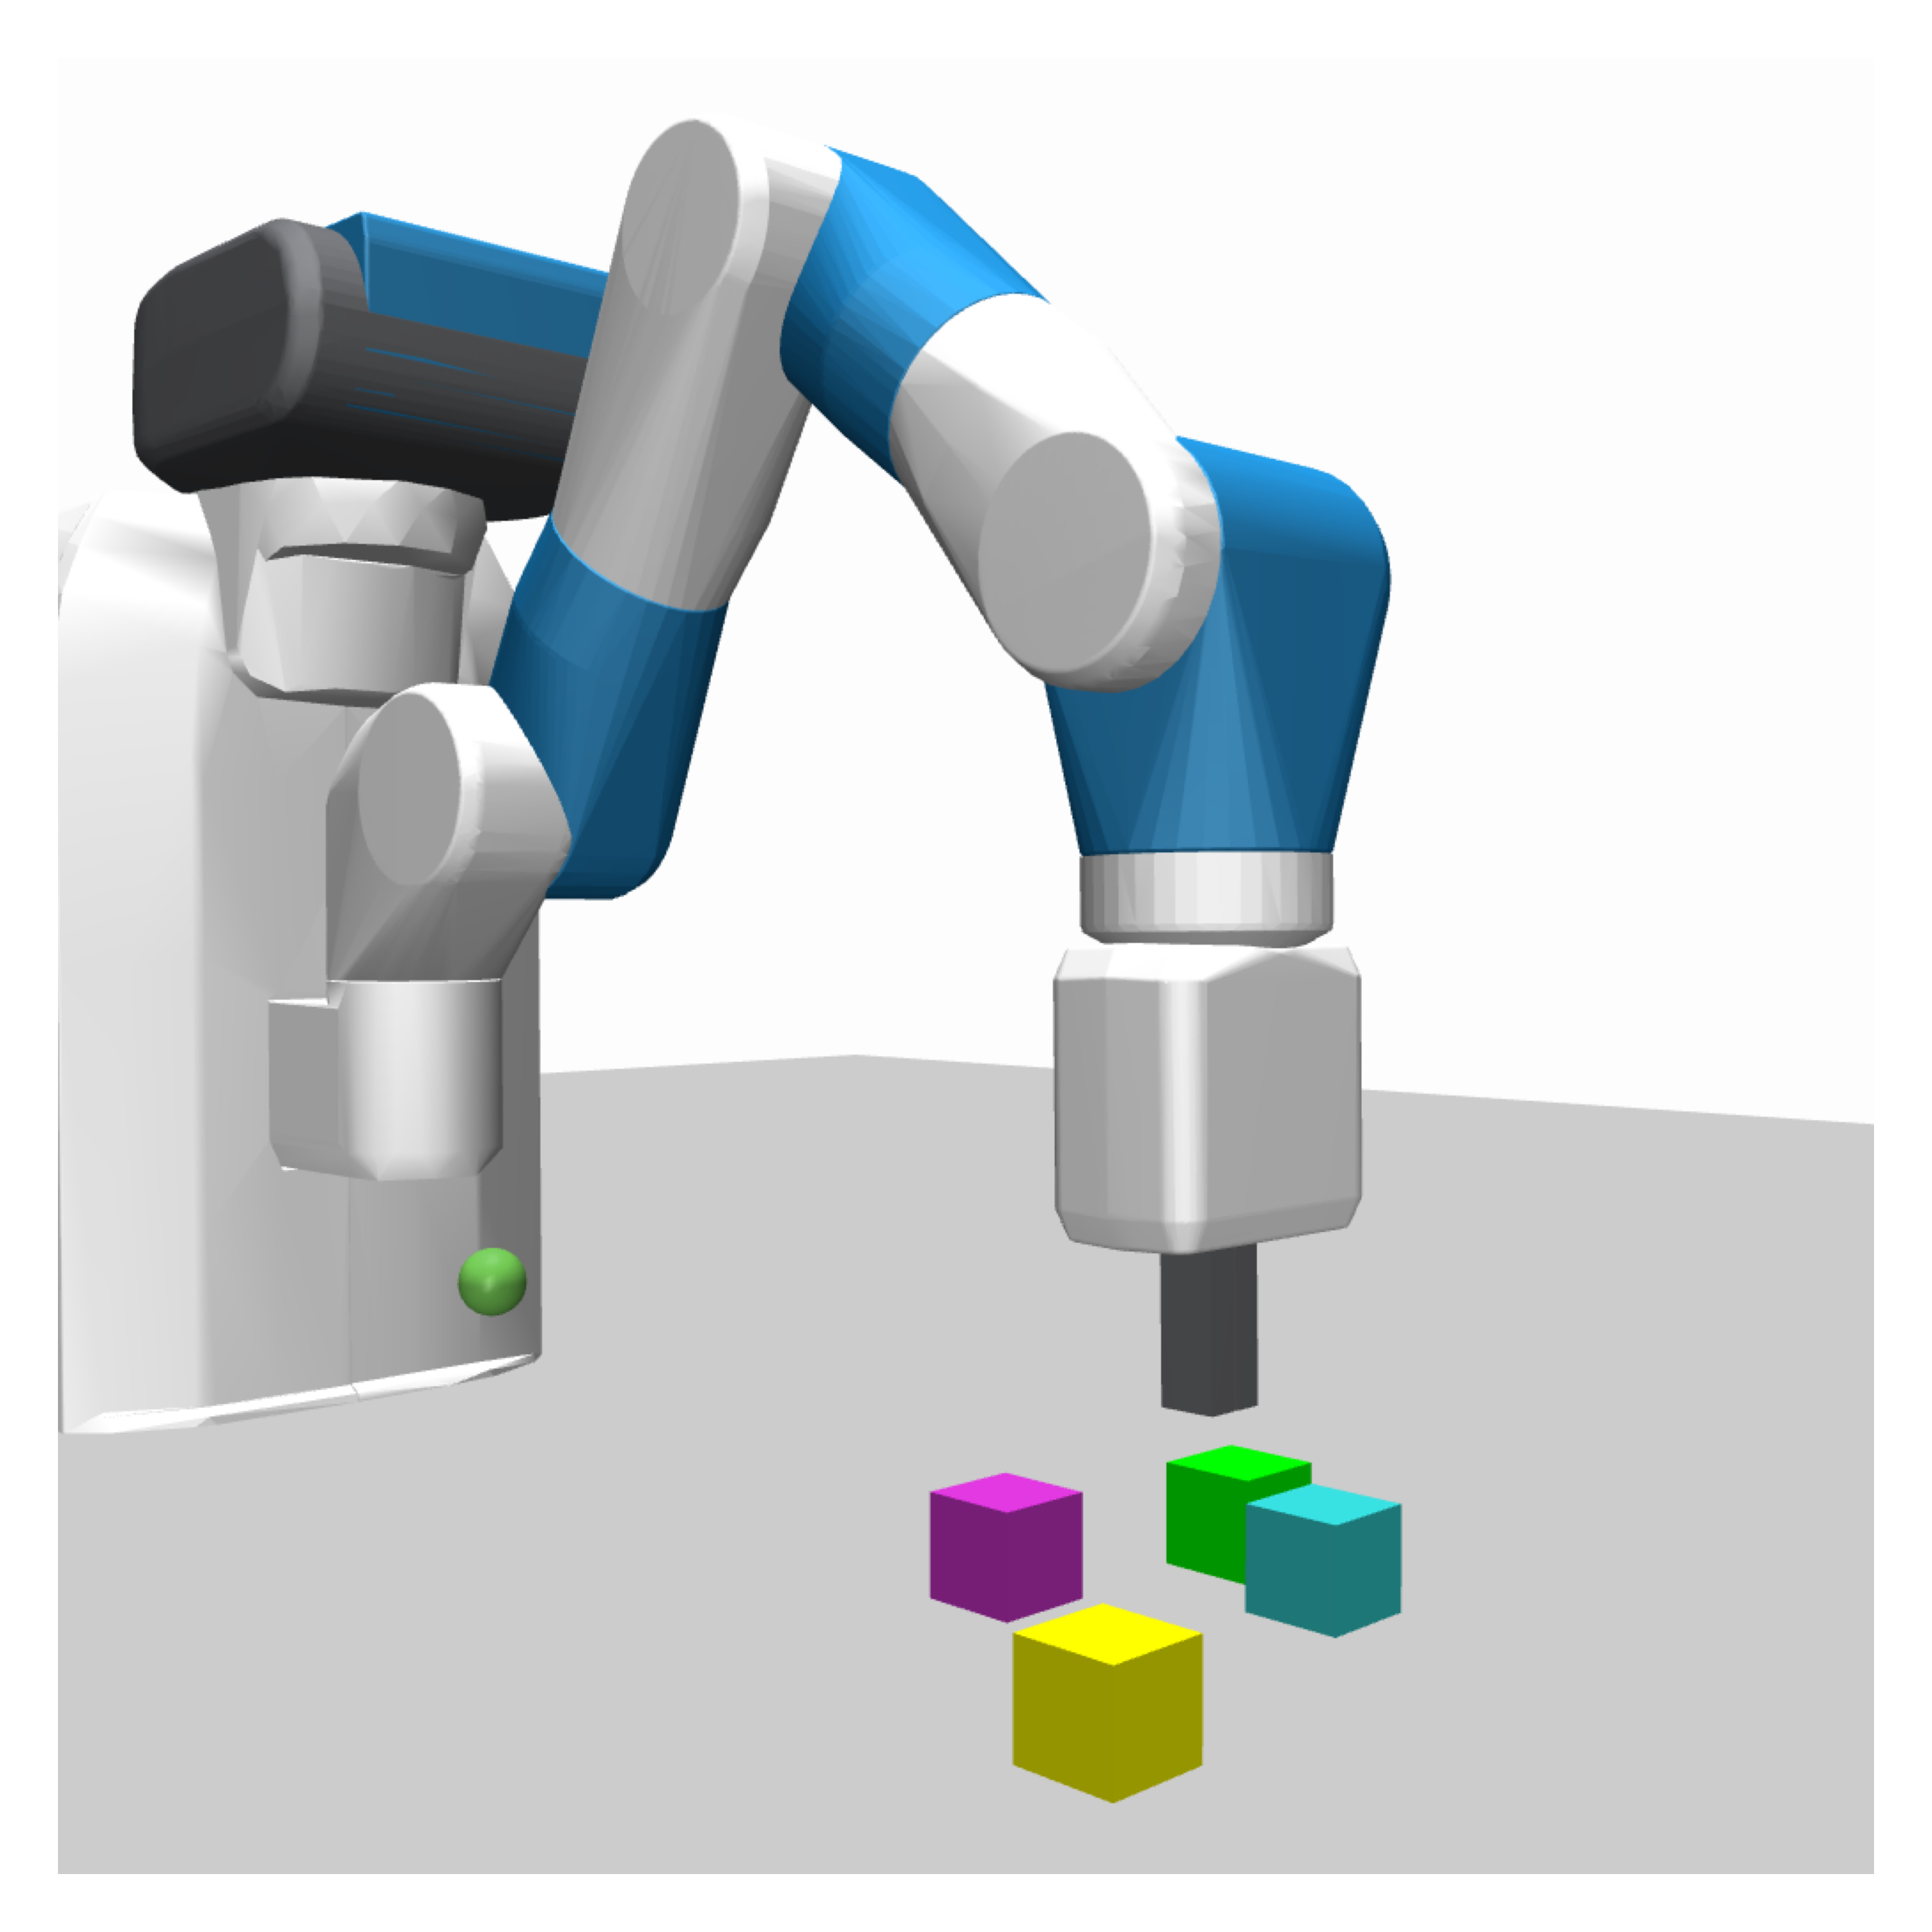
\includegraphics[width=\linewidth]{figures/env_4obj.png}
        \end{column}
        \begin{column}{0.7\textwidth}
            \textbf{Zero-shot performance on three challenging tasks:}
            \begin{itemize}
                \item Pick \& Place, Throw, and Flip tasks
                \item OPAX matches or exceeds state-of-the-art baselines
                \item Comparison includes CEEUS (previous SOTA for active exploration)
            \end{itemize}
            \vspace{0.5em}
            \textbf{Key finding:} OPAX scales effectively to high-dimensional continuous control problems while maintaining strong zero-shot generalization
        \end{column}
    \end{columns}
\end{frame}

\begin{frame}{Experiments: Fetch Pick \& Place Construction Results \hl{ben}}
    \centering
    \begin{figure}
        \centering
        \subfloat[Pick \& Place]{
            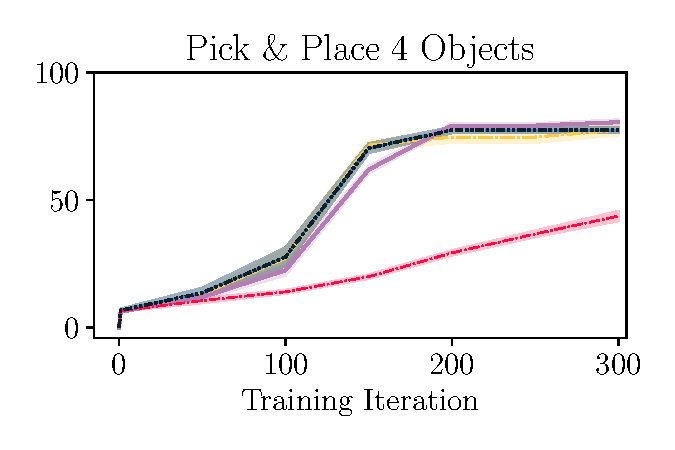
\includegraphics[width=.32\linewidth]{figures/construction_pp4_success_monotonous.pdf}
        }
        \subfloat[Throw]{
            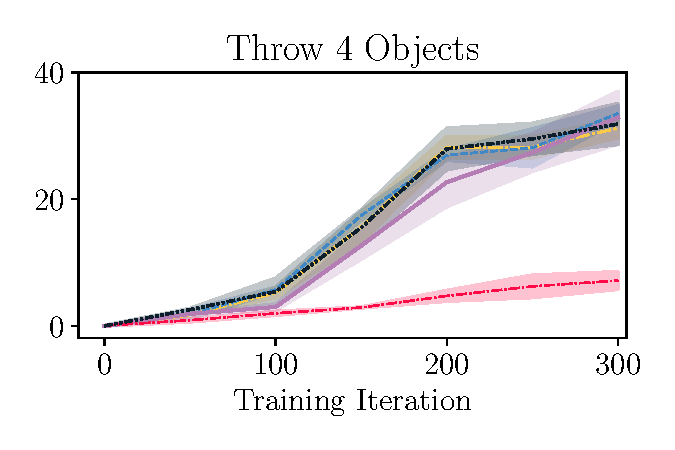
\includegraphics[width=.32\linewidth]{figures/construction_throw4_success_monotonous.pdf}
        }
        \subfloat[Flip]{
            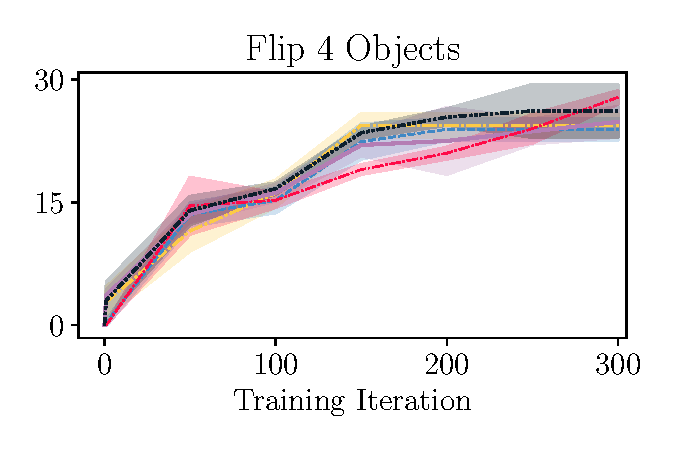
\includegraphics[width=.32\linewidth]{figures/construction_flip4_success_monotonous.pdf}
        }\\
        
\includegraphics[width=.6\linewidth]{figures/legend_updated.pdf}
    \end{figure}
    
    \begin{itemize}
        \item \textbf{OPAX} performs on par with or better than all baselines including CEEUS (state-of-the-art)
        \item Success rates evaluated via zero-shot planning with learned models
        \item Demonstrates scalability to high-dimensional (58D) continuous control
    \end{itemize}
\end{frame}

\begin{frame}{Key Findings \hl{ben}}
    \begin{itemize}
        \item \textbf{Sample Efficiency:}
        \begin{itemize}
            \item OPAX often reaches target performance with fewer environment interactions
            \item Active exploration methods significantly outperform random exploration
        \end{itemize}
        \pause
        \item \textbf{Generalization:}
        \begin{itemize}
            \item OPAX matches H-UCRL on trained tasks
            \item Significantly outperforms H-UCRL on unseen tasks (e.g., Cheetah run backward, Swimmer go away)
            \item Task-specific methods fail to explore regions irrelevant to their training reward
        \end{itemize}
        \pause
        \item \textbf{Scalability:}
        \begin{itemize}
            \item Successful application to high-dimensional Fetch task (58D) using PEs and MPC
            \item Performance on par with CEEUS (previous state-of-the-art for active exploration)
        \end{itemize}
        \pause
        \item \textbf{Objective Robustness:}
        \begin{itemize}
            \item Log-uncertainty objective (Eq. 6) performs similarly to simpler sum-of-uncertainties (OPAX-SUM)
            \item Core benefit comes from optimistic planning rather than specific reward formulation
        \end{itemize}
    \end{itemize}
\end{frame}

% --- Section 6: Discussion & Conclusion ---
\section{Discussion \& Conclusion}

\begin{frame}{Key Contributions and Impact \hl{ben}}
    \begin{columns}[T]
        \begin{column}{0.5\textwidth}
            \textbf{What OPAX Achieves:}
            \begin{itemize}
                \item \alert{First} practical algorithm with theory for continuous nonlinear dynamics
                \item Strong zero-shot generalization to unseen tasks
                \item Scales to high-dimensional problems (58D)
                \item Matches/exceeds SOTA baselines
            \end{itemize}
        \end{column}
        \begin{column}{0.5\textwidth}
            \textbf{Why It Matters:}
            \begin{itemize}
                \item Moves beyond task-specific learning
                \item Enables true multi-task capabilities
                \item Foundation for continual learning agents
                \item Step towards general-purpose AI
            \end{itemize}
        \end{column}
    \end{columns}
    
    \vspace{0.5em}
    \begin{block}{Core Innovation}
        Applying \alert{optimism} to \alert{information gain} rather than rewards creates a principled exploration strategy that builds comprehensive world models
    \end{block}
\end{frame}

\begin{frame}{Open Challenges and Future Work \hl{ben}}
    \begin{columns}[T]
        \begin{column}{0.48\textwidth}
            \textbf{Current Limitations:}
            \begin{itemize}
                \item Computationally expensive optimistic planning
                \item Requires well-calibrated uncertainty
                \item Limited to fully observed MDPs
                \item Pure exploration (no task integration)
            \end{itemize}
        \end{column}
        \begin{column}{0.48\textwidth}
            \textbf{Exciting Directions:}
            \begin{itemize}
                \item Amortized optimistic planning
                \item Robust uncertainty estimation
                \item Extension to POMDPs
                \item Exploration-exploitation balance
            \end{itemize}
        \end{column}
    \end{columns}
    
    \vspace{0.5em}
    \begin{alertblock}{Take-Home Message}
        OPAX demonstrates that \textbf{information-driven exploration} with \textbf{optimistic planning} can efficiently learn accurate, generalizable dynamics models – a crucial step towards truly adaptive AI systems.
    \end{alertblock}
\end{frame}

% --- Bibliography ---
\begin{frame}[allowframebreaks]{References} % allowframebreaks allows bibliography to span multiple slides if needed
    \printbibliography
\end{frame}

% --- Closing Slide ---
\begin{closingframe}

    \begin{center}
        \begin{minipage}{1\textwidth}
            \textbf{Chung-En Tsai}\hfill
            \textit{\email{chtsai@ethz.ch}}
            
            \vspace{0.25em}
            
            \textbf{Ben Bullinger}\hfill\textit{\email{bben@ethz.ch}}
        \end{minipage}
    \end{center}

    \vfill

    \begin{columns}
		\begin{column}{\textwidth}
            ETH Zurich\\
            Department of Computer Science
		\end{column}
	\end{columns}

\end{closingframe}

\end{document}

% --- Dummy references.bib file content ---
/*
@inproceedings{sukhija2023optimistic,
  title={Optimistic Active Exploration of Dynamical Systems},
  author={Sukhija, Bhavya and Treven, Lenart and Sancaktar, Cansu and Blaes, Sebastian and Coros, Stelian and Krause, Andreas},
  booktitle={Advances in Neural Information Processing Systems},
  volume={36},
  pages={45869--45883},
  year={2023},
  url={https://proceedings.neurips.cc/paper_files/paper/2023/file/a4a4cdab45ef4883ed66e49785819a94-Paper-Conference.pdf}
}

% Add other citations from the report if needed, e.g.:
@inproceedings{chua2018deep,
  title={Deep reinforcement learning in a handful of trials using probabilistic dynamics models},
  author={Chua, Kurtland and Calandra, Roberto and McAllister, Rowan and Levine, Sergey},
  booktitle={Advances in neural information processing systems},
  volume={31},
  year={2018}
}

@article{kakade2020information,
  title={Information theoretic regret bounds for reinforcement learning},
  author={Kakade, Sham M and Dann, Christoph and Krishnamurthy, Akshay},
  journal={arXiv preprint arXiv:2006.05211},
  year={2020}
}

@inproceedings{lakshminarayanan2017simple,
  title={Simple and scalable predictive uncertainty estimation using deep ensembles},
  author={Lakshminarayanan, Balaji and Pritzel, Alexander and Blundell, Charles},
  booktitle={Advances in neural information processing systems},
  volume={30},
  year={2017}
}

@inproceedings{haarnoja2018soft,
  title={Soft actor-critic: Off-policy maximum entropy deep reinforcement learning with a stochastic actor},
  author={Haarnoja, Tuomas and Zhou, Aurick and Abbeel, Pieter and Levine, Sergey},
  booktitle={International conference on machine learning},
  pages={1861--1870},
  year={2018},
  organization={PMLR}
}

@inproceedings{curi2020hucrl,
    title =        {{H-UCRL}: Hybrid Uncertainty Estimation for Model-Based {RL}},
    author =       {Curi, Sebastian and Berkenkamp, Felix and Krause, Andreas},
    booktitle =    {Proceedings of the 37th International Conference on Machine Learning},
    pages =        {2224--2233},
    year =         {2020},
    volume =       {119},
    series =       {Proceedings of Machine Learning Research},
    month =        {13--18 Jul},
    publisher =    {PMLR},
}

@inproceedings{li2020generalized,
  title={Generalized Hindsight for Long-Horizon Visuomotor Reinforcement Learning},
  author={Li, Alexander and Pong, Vitchyr H and Florence, Phillip and Agrawal, Pulkit and Levine, Sergey},
  booktitle={Robotics: Science and Systems (RSS)},
  year={2020}
}

@article{chaloner1995bayesian,
  title={Bayesian experimental design: A review},
  author={Chaloner, Kathryn and Verdinelli, Isabella},
  journal={Statistical Science},
  pages={273--304},
  year={1995},
  publisher={JSTOR}
}

@inproceedings{wagenmaker2023certainty,
  title={Certainty-equivalent exploration in latent dynamics models},
  author={Wagenmaker, Andrew J and Ma, Yifan and Boots, Byron},
  booktitle={Conference on Robot Learning},
  pages={1403--1413},
  year={2023},
  organization={PMLR}
}

*/
